\clearpage
\chapter{Results}
\section{Result experiment decreasing amount}
    \clearpage
    \begin{figure}[H]
        \centering
        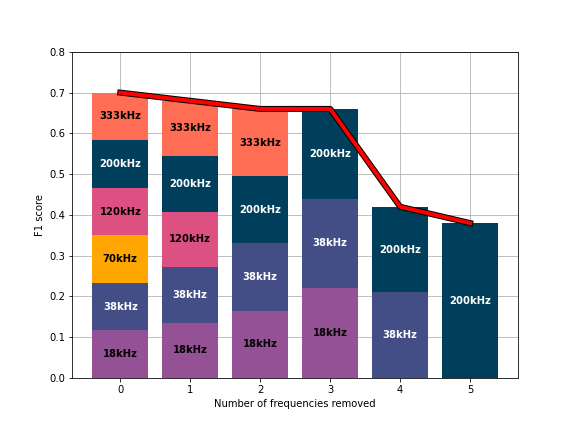
\includegraphics[scale=0.8]{figures/ta_vekk_frekvenser.png}
        \caption{Overview of the greedy frequency test from all to one single frequency. The red line is the best F1 score during the tests at each stage. Colored blocks indicate the frequencies that resulted in the previously mentioned score.}
      	\medskip 
        \label{decrease_amount_fig}
    \end{figure}

\section{Result experiment increasing amount}
    \clearpage
    \begin{figure}[H]
        \centering
        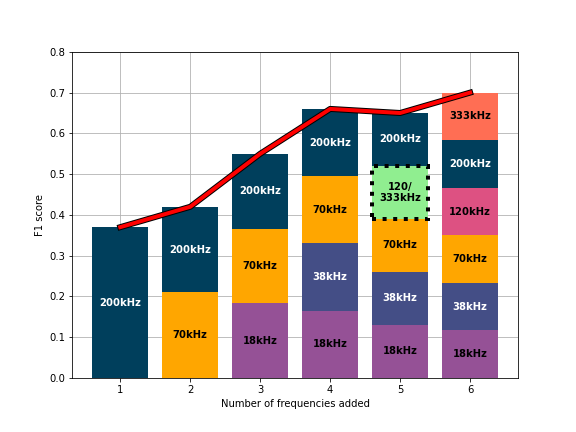
\includegraphics[scale=0.8]{figures/legge_til_frekvenser.png}
        \caption{Overview of the greedy frequency test from one frequency to all. The red line is the best F1 score during the tests at each stage. Colored blocks indicate the frequencies that resulted in the previously mentioned score. Where the number of frequencies are 5, there is a light green block indicating that both frequencies got the same F1 score.}
      	\medskip 
        \label{dincrease_amount_fig}
    \end{figure}